\begin{center}
	
	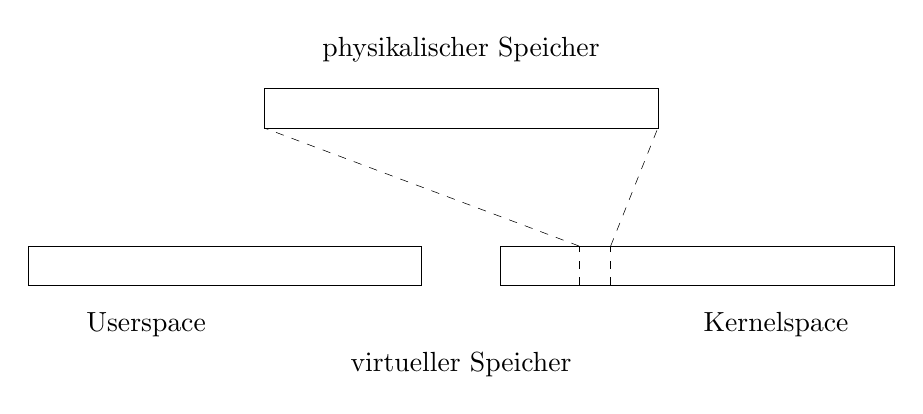
\begin{tikzpicture}
	% physikalischer Speicher
	\node[] at (5.5,3) {physikalischer Speicher};
	\draw[step=0.5cm,very thin] (3,2) rectangle (8,2.5);
	
	% virtueller Speicher
	\node[] at (5.5,-1) {virtueller Speicher};
	\node[] at (1.5,-0.5) {Userspace};
	\node[] at (9.5,-0.5) {Kernelspace};
	\draw[step=0.5cm,very thin] (0,0) rectangle (5,0.5);
	\draw[step=0.5cm,very thin] (6,0) rectangle (11,0.5);
	
	% direct Mapping
	\draw[step=0.5cm,very thin, dashed] (7,0) -- (7,0.5);
	\draw[step=0.5cm,very thin, dashed] (7.4,0) -- (7.4,0.5);
	\draw[step=0.5cm,very thin, dashed] (7,0.5) -- (3,2);
	\draw[step=0.5cm,very thin, dashed] (7.4,0.5) -- (8,2);
	
	% user page
	% \draw[red, very thin, dashed] (3,0) -- (3,0.5);
	% \draw [red, ->]  (3,0.5) to [out=90,in=270,looseness=1.3] (5,2);
	% \draw[red, very thin, dashed] (5,2) -- (5,2.5);
	% \draw[green, very thin, dashed] (3,0) -- (3,0.5);
	% \draw [green, ->]  (3,0.5) to [out=90,in=270,looseness=1.3] (5,2);
	% \draw[green, very thin, dashed] (5,2) -- (5,2.5);
	
	% \draw [->]  (7,0.5) to [out=90,in=270,looseness=0.2] (3,2);
	% \draw [->]  (7.03,0.5) to [out=90,in=270,looseness=0.2] (3.1,2);
	% \draw [->]  (7.06,0.5) to [out=90,in=270,looseness=0.2] (3.2,2);
	% \draw [->]  (7.14,0.5) to [out=90,in=270,looseness=0.2] (4,2);
	% \draw [green, ->]  (7.22,0.5) to [out=90,in=270,looseness=0.2] (5,2);
	
	
	\end{tikzpicture}
	
\end{center}